% =====================================================================
%  CHƯƠNG 3 — NGHIÊN CỨU THỰC NGHIỆM VÀ HIỆN THỰC HỆ THỐNG
% =====================================================================
\chapter{Nghiên cứu thực nghiệm và hiện thực hệ thống}

Mọi con số trong chương này lấy trực tiếp từ artifact sinh bởi mã nguồn
(\texttt{reports/results/*.json}) và tái lập được bằng \texttt{python -m scripts.run\_all}.

\section{Pipeline xử lý dữ liệu SEC XBRL}

\subsection{Tải và chọn corpus}

Dữ liệu thô được tải bằng \texttt{scripts/crawl\_sec.py}: mỗi công ty là một file
\texttt{companyfacts} 5--8 MB, kèm delay 0,15 giây giữa các request để tôn trọng giới hạn tần suất
của SEC. Hash SHA-256 của từng file được ghi vào \texttt{data/sec/downloads.json} để về sau đối
chiếu được là file không bị sửa tay.

Từ 20 công ty ban đầu, nhóm giữ 8 công ty thoả hai điều kiện: tối thiểu 32 quý báo cáo và đủ 16 chỉ
tiêu chuẩn. Danh sách công ty bị loại kèm lý do cụ thể nằm trong
\texttt{data/retail-expanded/corpus.json}.

\begin{table}[H]
\centering
\caption{Corpus 8 doanh nghiệp bán lẻ và số quý dữ liệu}
\label{tab:corpus}
\begin{tabular}{|l|l|r|l|r|}
\hline
\textbf{Ticker} & \textbf{Công ty} & \textbf{Số quý} & \textbf{Năm tài chính} & \textbf{Tỉ lệ nhãn = 1} \\
\hline
WMT  & Walmart            & 48 & FY2015--FY2026 & 100\% \\
HD   & The Home Depot     & 44 & FY2015--FY2026 & 100\% \\
LOW  & Lowe's             & 44 & FY2015--FY2026 & 100\% \\
ROST & Ross Stores        & 44 & FY2015--FY2026 & 5\%   \\
DG   & Dollar General     & 32 & FY2018--FY2026 & 55\%  \\
ORLY & O'Reilly Automotive& 44 & FY2015--FY2026 & 91\%  \\
DKS  & Dick's Sporting    & 44 & FY2015--FY2026 & 12\%  \\
FIVE & Five Below         & 32 & FY2018--FY2026 & 19\%  \\
\hline
\end{tabular}
\end{table}

\subsection{Bóc tách chỉ tiêu từ companyfacts}

Hàm \texttt{derive\_cell} trong \texttt{scripts/prepare\_sec.py} tái tạo từng ô dữ liệu theo thứ tự
ưu tiên: thử các tag theo \texttt{TAG\_PRIORITY}, rồi áp một trong bốn phương pháp — số dư cuối kỳ
(\texttt{instant}), fact đúng quý (\texttt{reported\_quarter}/\texttt{reported\_first\_quarter}),
luỹ kế trừ luỹ kế (\texttt{current\_ytd\_minus\_previous\_ytd}), hoặc để trống (\texttt{absent}). Mã
nguồn không bao giờ "đoán" giá trị: thiếu fact thì trả \texttt{None} và ghi method \texttt{absent}.
Khi một kỳ có nhiều bản công bố (nộp lại báo cáo), hàm \texttt{\_published} chọn bản công bố SỚM
NHẤT đã có trước thời điểm ra quyết định.

Một điểm phải xử lý riêng là thẻ \texttt{liabilities}: chỉ 39\% số quý có tag này, có công ty dưới
16\%. Nếu bỏ qua, hai đặc trưng \texttt{debt\_to\_assets} và \texttt{debt\_to\_equity} sẽ thiếu ở
phần lớn mẫu và mô hình mất hẳn thông tin đòn bẩy. Khóa luận suy nợ phải trả từ đẳng thức kế toán
$\text{nợ} = \text{tổng tài sản} - \text{vốn chủ sở hữu}$ khi thiếu tag, rồi đối chiếu lại 124 quý có
tag: 122 quý khớp tuyệt đối, 2 quý lệch do nộp lại báo cáo.

\subsection{Kết quả kiểm chứng nguồn gốc dữ liệu}

Tổng cộng 16 chỉ tiêu $\times$ 332 quý $=$ 5.312 ô dữ liệu. Bước kiểm chứng
(\texttt{scripts/verify\_provenance.py}) mở lại từng snapshot và tra ngược từng ô; kết quả ở
Bảng~\ref{tab:provenance}.

\begin{table}[H]
\centering
\caption{Kiểm chứng nguồn gốc dữ liệu với snapshot SEC công khai}
\label{tab:provenance}
\begin{tabular}{|l|r|}
\hline
\textbf{Phép kiểm} & \textbf{Số lượng} \\
\hline
File SEC đã băm SHA-256            & 20 \\
Hash lệch so với registry          & 0 \\
Ô dữ liệu (quý $\times$ chỉ tiêu)  & 5.312 \\
Ô không có fact ở SEC (để \texttt{null}) & 703 \\
Ô có fact, đối chiếu ngược được    & 4.609 \\
Fact không tồn tại trong SEC       & 0 \\
Ô không có fact nhưng vẫn có số    & 0 \\
\hline
\end{tabular}
\end{table}

\subsection{Định nghĩa nhãn}

Nhãn gốc \texttt{is\_distressed} là trạng thái của quý target. Điều đáng chú ý là nhãn này KHÔNG tái
tạo được từ 16 chỉ tiêu công bố: thử 9 quy tắc kế toán đơn giản, quy tắc khớp cao nhất
(\texttt{stress\_signals} $\geq 1$ tín hiệu) chỉ đạt 74,7\%, còn các quy tắc đơn chỉ tiêu chỉ đạt
39--65\%. Khóa luận xử lý bằng hai cách: (i) kiểm chứng độ nhạy với các định nghĩa nhãn tái lập được
(mục~\ref{sec:nhan}); (ii) ghi rõ giới hạn thay vì che đi.

Nhãn quy tắc tái lập được định nghĩa trong \texttt{forecasting/labels.py}: gán 1 nếu quý target có
ít nhất $k$ tín hiệu căng thẳng trong sáu tín hiệu — lỗ ròng, dòng tiền hoạt động âm, lỗ hoạt động,
vốn lưu động âm, vốn chủ sở hữu âm, và doanh thu giảm hơn 5\% so với cùng kỳ. Tín hiệu thiếu dữ liệu
được coi là không xảy ra (bảo thủ, không suy diễn).

\subsection{Chia tập và dải purge}

Chính sách chia tập theo thứ tự thời gian trong từng công ty: 8 quý cuối là test, 4 quý liền trước là
validation, phần còn lại là train. Giữa các tập có dải purge: mỗi công ty bỏ ra 1 quý ngay trước
validation và 1 quý ngay sau validation để tránh rò rỉ nhãn do cửa sổ lịch sử chồng lấn. Kết quả:
train 212 mẫu, validation 32, test 64, purged 16 (Bảng~\ref{tab:split}).

\begin{table}[H]
\centering
\caption{Số mẫu và tỉ lệ lớp theo từng tập}
\label{tab:split}
\begin{tabular}{|l|r|r|r|r|}
\hline
\textbf{Tập} & \textbf{n} & \textbf{Lớp 1} & \textbf{Lớp 0} & \textbf{IR} \\
\hline
train      & 212 & 132 (62,3\%) & 80 (37,7\%)  & 1,65 \\
validation & 32  & 21 (65,6\%)  & 11 (34,4\%)  & 1,91 \\
test       & 64  & 38 (59,4\%)  & 26 (40,6\%)  & 1,46 \\
purged     & 16  & 11 (68,8\%)  & 5 (31,2\%)   & 2,20 \\
\hline
\end{tabular}
\end{table}

\section{Trích xuất đặc trưng}

\subsection{Đặc điểm dữ liệu quan sát trước khi tạo đặc trưng}

Hai đặc điểm định hình toàn bộ thiết kế phía sau. Thứ nhất, mất cân bằng lớp ở cấp mẫu chỉ ở mức nhẹ
(lớp suy giảm chiếm 62,3\% train, IR $= 1{,}65$), nhưng ở cấp công ty rất nặng: HD, LOW, WMT có
100\% quý mang nhãn 1; ROST chỉ 4,7\%. Điều này có nghĩa nhãn gần như là thuộc tính của từng công ty,
nên mọi đánh giá phải chia theo nhóm công ty. Thứ hai, phân phối các tỷ số lệch mạnh: trong 14 tỷ
số, 6 tỷ số có $|\text{skew}| > 1$, nặng nhất là \texttt{debt\_to\_equity} (skew $-14{,}9$) với
30,6\% giá trị nằm ngoài khoảng IQR.

\begin{figure}[H]
\centering
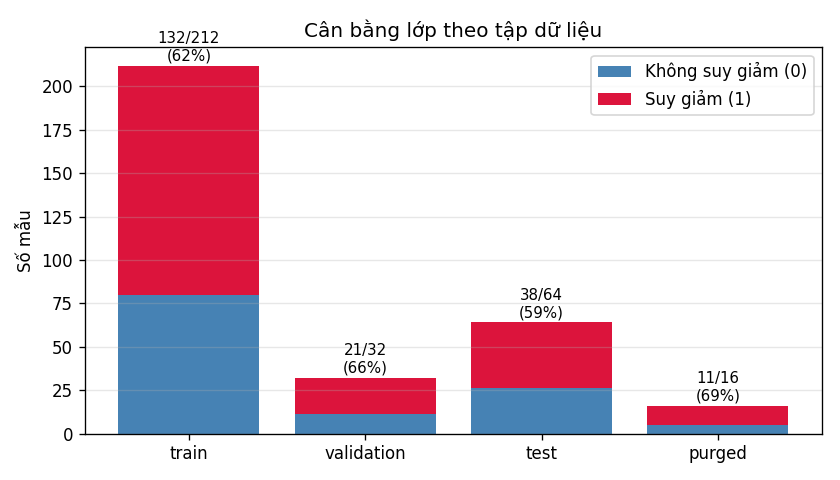
\includegraphics[width=0.78\textwidth]{figures/class_balance.png}
\caption{Cân bằng lớp theo tập dữ liệu}
\label{fig:class_balance}
\end{figure}

\begin{figure}[H]
\centering
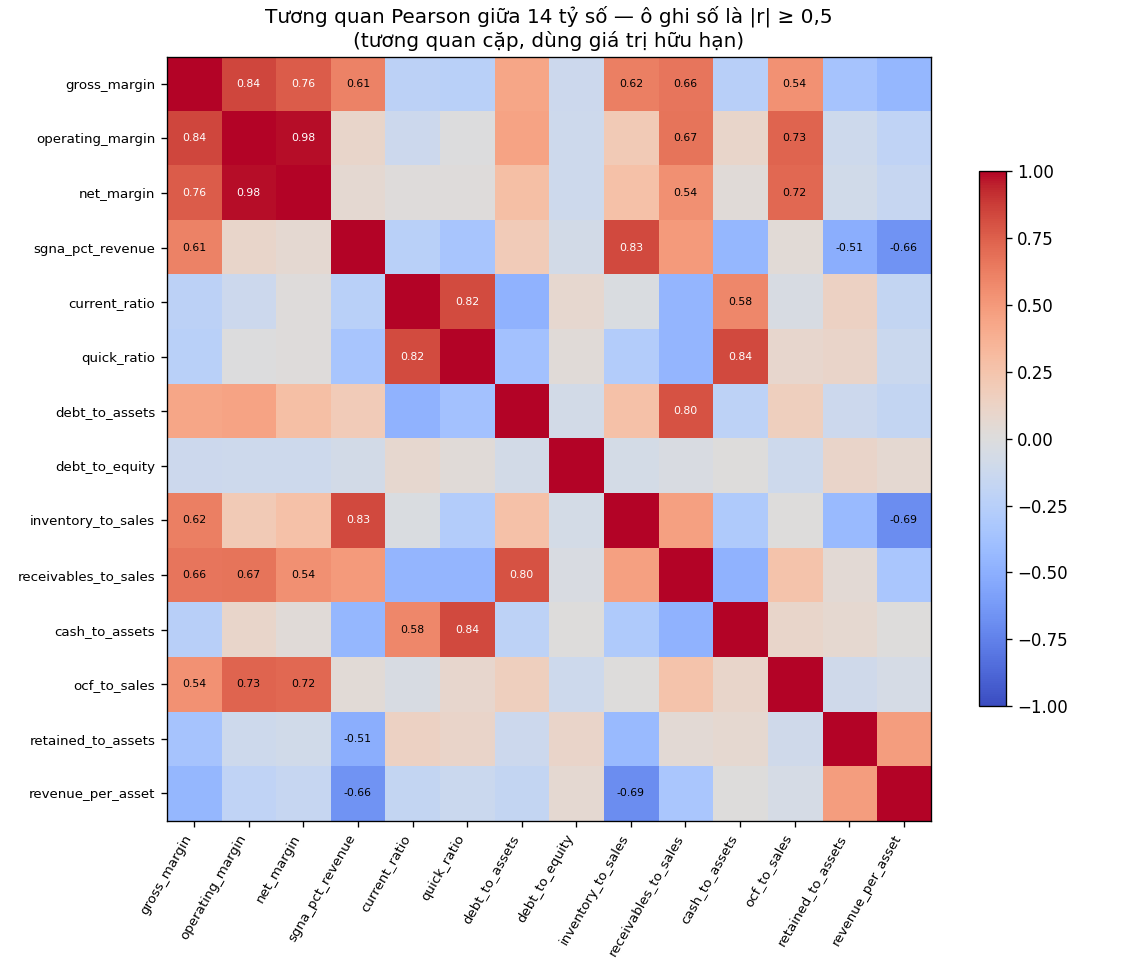
\includegraphics[width=0.78\textwidth]{figures/ratio_correlation.png}
\caption{Tương quan giữa các tỷ số tài chính}
\label{fig:ratio_corr}
\end{figure}

\subsection{Mười bốn tỷ số tài chính}

Các tỷ số (từ điển \texttt{RATIOS} trong \texttt{forecasting/config.py}) chia bốn nhóm kinh tế:

\begin{itemize}
\item \textbf{Thanh khoản:} \texttt{current\_ratio} $=$ tài sản ngắn hạn / nợ ngắn hạn;
      \texttt{quick\_ratio} $=$ (tài sản ngắn hạn $-$ hàng tồn kho) / nợ ngắn hạn.
\item \textbf{Đòn bẩy:} \texttt{debt\_to\_assets} $=$ nợ / tổng tài sản; \texttt{debt\_to\_equity}
      $=$ nợ / vốn chủ sở hữu.
\item \textbf{Sinh lời:} \texttt{gross\_margin} $=$ (doanh thu $-$ giá vốn) / doanh thu;
      \texttt{operating\_margin} $=$ lợi nhuận hoạt động / doanh thu; \texttt{net\_margin} $=$ lợi
      nhuận ròng / doanh thu; \texttt{retained\_to\_assets} $=$ lợi nhuận giữ lại / tổng tài sản.
\item \textbf{Hiệu quả hoạt động:} \texttt{inventory\_to\_sales}, \texttt{receivables\_to\_sales},
      \texttt{revenue\_per\_asset}, \texttt{ocf\_to\_sales}, \texttt{sgna\_pct\_revenue},
      \texttt{cash\_to\_assets}.
\end{itemize}

Mỗi tỷ số được đưa vào mô hình ở hai dạng: giá trị của quý gần nhất (\texttt{*\_latest}) và mức thay
đổi so với cùng kỳ năm trước (\texttt{*\_yoy}), tức $14 \times 2 = 28$ cột.

\subsection{Tăng trưởng, cấu trúc vốn và đặc trưng đường đi}

Nhóm tăng trưởng gồm 10 cột \texttt{*\_yoy\_growth} cho các chỉ tiêu chính. Nhóm cấu trúc vốn có
\texttt{working\_capital\_to\_assets}. Nhóm đường đi (\texttt{path}) là phần thiết kế riêng cho bài
toán này: vì suy giảm tài chính là một quá trình, khóa luận đưa vào cực trị xấu nhất trong cửa sổ và
số quý âm liên tiếp — \texttt{current\_ratio\_min\_window}, \texttt{ocf\_to\_sales\_min\_window},
\texttt{net\_margin\_min\_window}, \texttt{revenue\_drawdown\_window},
\texttt{negative\_ni\_streak}, \texttt{negative\_ocf\_streak}.

\begin{table}[H]
\centering
\caption{Cấu trúc 47 đặc trưng theo nhóm}
\label{tab:feature_groups}
\begin{tabular}{|l|r|l|}
\hline
\textbf{Nhóm} & \textbf{Số cột} & \textbf{Nội dung} \\
\hline
ratios\_latest & 14 & 14 tỷ số tại quý gần nhất \\
ratios\_yoy    & 14 & Mức thay đổi so với cùng kỳ \\
growth         & 10 & Tăng trưởng YoY của 10 chỉ tiêu chính \\
structure      & 1  & working\_capital\_to\_assets \\
stress         & 2  & distress\_quarters\_in\_window, revenue\_cv \\
path           & 6  & Cực trị xấu nhất + số quý âm liên tiếp \\
\hline
\textbf{Tổng}  & \textbf{47} & \\
\hline
\end{tabular}
\end{table}

\subsection{Xử lý giá trị khuyết và ngoại lai}

Giá trị khuyết giữ nguyên dạng NaN qua tầng đặc trưng, rồi xử lý bên trong pipeline bằng
\texttt{SimpleImputer(strategy='median')}, với median tính chỉ trên train. Với ngoại lai, khóa luận
thử \texttt{Winsorizer} (clip theo IQR hoặc P1--P99, ngưỡng học từ train) như một biến thể và báo
cáo kết quả âm: trên đúng mô hình được chốt (Random Forest), winsorize IQR cải thiện AP
cross-company chỉ $+0{,}13$ điểm \% (0,9590 so với 0,9577) — nằm trong khoảng nhiễu của 244 mẫu
out-of-fold. Vì vậy pipeline chính giữ không winsorize cho đơn giản và dễ diễn giải; winsorize chỉ
dùng như một ablation. Kết quả tương tự với lựa chọn scaler: \texttt{StandardScaler} và
\texttt{RobustScaler} chênh nhau dưới 0,5 điểm \% AP cross-company.

\section{Thiết kế mô hình học máy}
\label{sec:models}

\subsection{Bốn họ mô hình}

Khóa luận cố tình chọn bốn họ mô hình khác nhau về cơ chế học để trả lời câu hỏi "bài toán cần loại
giả thuyết nào", thay vì thử nhiều biến thể của cùng một họ: tuyến tính (Logistic Regression),
bagging cây (Random Forest), boosting cây (HistGradientBoosting) và mạng nơ-ron phi tuyến không dựa
trên cây (MLP). Toàn bộ dùng thư viện \texttt{scikit-learn}; pipeline chính không dùng
\texttt{xgboost}/\texttt{lightgbm}.

\begin{table}[H]
\centering
\caption{Siêu tham số của bốn họ mô hình}
\label{tab:hyperparams}
\begin{tabular}{|l|l|p{7.4cm}|}
\hline
\textbf{Mô hình} & \textbf{Lớp scikit-learn} & \textbf{Siêu tham số mặc định} \\
\hline
Logistic Regression & LogisticRegression & max\_iter=2000, C=0,1 \\
Random Forest & RandomForestClassifier & n\_estimators=300, max\_depth=6,
min\_samples\_leaf=2, class\_weight=balanced\_subsample \\
HistGradientBoosting & HistGradientBoostingClassifier & max\_iter=300, learning\_rate=0,05,
max\_depth=3, l2\_regularization=1,0, class\_weight=balanced \\
MLP & MLPClassifier & hidden\_layer\_sizes=32, alpha=1e-3, learning\_rate\_init=1e-3,
early\_stopping=True \\
\hline
\end{tabular}
\end{table}

Lưu ý kỹ thuật với mất cân bằng: \texttt{RandomForestClassifier} và
\texttt{HistGradientBoostingClassifier} nhận \texttt{class\_weight} nên trọng số lớp được truyền
trực tiếp. \texttt{MLPClassifier} không có \texttt{class\_weight}, nên mất cân bằng được xử lý bằng
ngưỡng/cost-sensitive ở tầng đánh giá thay vì nhồi trọng số giả vào mô hình.

\subsection{Pipeline và kiểm soát rò rỉ dữ liệu}

Mỗi mô hình là một \texttt{sklearn.pipeline.Pipeline}:
\texttt{[winsorize] $\rightarrow$ SimpleImputer(median) $\rightarrow$ [scaler] $\rightarrow$ model}
(hàm \texttt{make\_model} trong \texttt{forecasting/models.py}). Đặt bước impute và scale bên trong
Pipeline có tác dụng chặn rò rỉ: thống kê impute/scale chỉ được \texttt{fit} trên train, và khi kiểm
định chéo chỉ trên fold-train. Scaler mặc định là \texttt{StandardScaler} cho mô hình tuyến
tính/MLP và \texttt{none} cho mô hình cây. \texttt{RANDOM\_SEED = 42} được cố định để tái lập.

\subsection{Quy tắc chọn mô hình}

Nếu chọn mô hình theo AUROC in-domain, kết quả sẽ bị chi phối bởi việc "nhớ mặt công ty" — baseline
ticker-prior đạt AUROC 0,986 (mục~\ref{sec:baseline}). Vì vậy quy tắc chọn theo thứ tự ưu tiên:
\textbf{AP cross-company} (GroupKFold trên train+validation) $\rightarrow$ best-F1(validation)
$\rightarrow$ AP(validation) $\rightarrow$ AUROC(validation) $\rightarrow$ gap overfit nhỏ nhất. Quy
tắc này được mã hoá tại \texttt{forecasting/train.py::\_rank} và ghi lại trong \texttt{summary.json}
để kiểm chứng được.

\subsection{Tinh chỉnh siêu tham số}

Tinh chỉnh dùng kiểm định chéo chia theo công ty (\texttt{GroupKFold}) và chọn theo AP, để không lặp
lại sai lầm chọn theo metric in-domain. Nhận xét trung thực: kết quả tinh chỉnh chênh lệch rất nhỏ
so với cấu hình mặc định — mô hình RF tốt nhất (\texttt{max\_depth=3, n\_estimators=500}) chỉ hơn
mặc định $+0{,}3$ điểm \% CV-AP; MLP hơn $+4{,}6$ điểm \% nhưng vẫn tụt hậu về cross-company. Vì
vậy mô hình triển khai giữ cấu hình mặc định (đơn giản, ít nguy cơ overfit do lựa chọn), và bảng
tinh chỉnh được giữ lại như bằng chứng là nhóm đã thử.

\begin{table}[H]
\centering
\caption{Tinh chỉnh siêu tham số, kiểm định chéo chia theo công ty}
\label{tab:tuning}
\begin{tabular}{|l|l|r|r|}
\hline
\textbf{Mô hình} & \textbf{Cấu hình tốt nhất} & \textbf{CV-AP} & \textbf{CV-AUROC} \\
\hline
logistic & C=0,01, class\_weight=None & 0,960 & 0,917 \\
random\_forest & max\_depth=3, min\_samples\_leaf=2, n\_estimators=500 & 0,989 & 0,976 \\
hist\_gradient\_boosting & learning\_rate=0,03, max\_depth=2, max\_iter=200 & 0,939 & 0,934 \\
mlp & alpha=1e-4, hidden\_layer\_sizes=64 & 0,845 & 0,750 \\
\hline
\end{tabular}
\end{table}


